\chapter{Feedback for Training Flight Tasks}
\label{chapter:aircraftfeedback}
% John A. Karasinski, Stephen K. Robinson
% Department of Mechanical and Aerospace Engineering, University of California, Davis

Portions of this chapter were originally published in the conference proceedings for the Human Factors and Ergonomics Society 2019~\citep{RN42}.

\section{Introduction}
Augmented feedback, information that relates an individual's performance to a desired performance, has been found to generally enhance motor learning in a wide variety of manual motor control tasks~\citep{salmoni_knowledge_1984}.
Many feedback modalities and implementations have been investigated in the literature, some of which have been found to be more effective than others.
One of the key aspects to successfully implementing feedback is knowing when to provide feedback to the participant.
Feedback can be provided concurrently, in real-time as the task is executed; or terminally, after the task is completed.
Visual concurrent feedback, for example, has been shown to greatly enhance motor learning as task complexity increases, while terminal feedback is better suited for tasks with low functional complexity~\citep{sigrist_augmented_2013}.
As \citeauthor{sigrist_augmented_2013} note in their review of augmented visual, auditory, haptic, and multimodal feedback, however, "[u]p to now, mostly low-dimensional, simple, and rather artificial labor tasks have been investigated even though, in real life, most motor tasks are multidimensional and complex."
Aircraft and spacecraft flight-control tasks are complex, multidimensional challenges for human manual control, and present both demanding learning requirements and high cognitive demands.
In the pursuit of improving pilot performance during training, several researchers have investigated the effects of adding visual and/or audio feedback to flight displays.
\citeauthor{doi:10.1518/001872096778940859} explored the use of auditory displays in a 3D flight task.
By adding auditory displays to the existing simulation, they were able to reduce search time in an aircraft location and tracking task.
Similarly, \citeauthor{doi:10.1207/s15327108ijap1403} showed that U.S. Air Force pilots could better maintain flight parameters and report reduced workload with the use of multisensory cueing.
Of the many studied feedback strategies, concurrent bandwidth feedback is among the most promising for complex tasks.
Concurrent bandwidth feedback is presented in real-time, during task execution, but only when some variable deviates outside of a defined bandwidth of acceptable values.
Researchers have used concurrent bandwidth feedback to study participants ability to learn to drive a vehicle, having found it to be effective at improving lane keeping~\citep{de_groot_effect_2011}.

At UC Davis, our recent experiments with concurrent bandwidth feedback in complex manual tasks have resulted in large improvements in human performance with an added benefit of reduced workload.
Our experiment with simulated spacecraft-piloting investigated the effects of concurrent bandwidth feedback on a complex, four-degree-of-freedom manually controlled on-orbit inspection task~\citep{karasinski_real-time_2017}.
We found that simple visual feedback on the controlled degrees of freedom improved initial and fully trained performance while reducing inferred and self-reported workload.
In fact, participants in the feedback group performed as well in their first trial as participants in the control group did after two hours of training.
Our recent work also includes an investigation into the effectiveness of concurrent bandwidth feedback for learning a 3D joystick-controlled tracking task in augmented reality~\citep{karasinski_evaluating_2019}.
This experiment investigated whether concurrent bandwidth feedback could teach participants to interpret 3D depth cues.
Our results suggested that participants who were exposed to visual concurrent bandwidth feedback early on sustained improved performance through the duration of the experiment compared to participants that began in a baseline condition without feedback.
Through these previous experiments, we have shown that concurrent bandwidth feedback can be effective at improving human performance for complex manual tasks.
The very complex spacecraft piloting experiment also showed large reductions in cognitive workload, though this effect was not observed in the 3D tracking experiment, which had much lower functional task complexity.
In the research reported here, we build upon our previous work and that in the literature by investigating an operationally relevant, joystick-commanded flight-control task with the objective of determining the effect of task complexity on the influence of concurrent bandwidth feedback.

In our current experiment, subjects controlled a simulated aircraft with realistic flight dynamics through a series of tasks of increasing functional complexity.
By allowing for multiple levels of functional complexity, we can investigate what level of complexity is required to observe changes in human performance and cognitive workload.
This experiment also investigated the effects of removing concurrent feedback after training to evaluate changes in performance and workload during participants' immediate retention.
The retention portion of the experiment was performed to investigate whether the guidance hypothesis, which states that consistent feedback during the acquisition phase of learning leads to a dependency on the feedback~\citep{salmoni_knowledge_1984}.

\section{Method}
\subsection{Task}
\subsubsection{Control Modes}
Participants were tasked with flying a simulated Boeing 747 aircraft in three control modes. In order of increasing degrees of freedom and functional complexity, these three control modes were:
\begin{itemize}
    \item[\textbf{P}] Pitch only (low complexity)
    \item[\textbf{PR}] Pitch and Roll (moderate complexity)
    \item[\textbf{PRA}] Pitch, Roll and Altitude (significant complexity)
\end{itemize}
Depending on the control mode, participants were required to use a joystick to null disturbances in pitch, roll, and/or to maintain a constant altitude.
Participants were informed that all three tasks were equally important, and to try not to neglect or prioritize individual tasks.

Each participant completed a total of 36 trials; 12 in each of the three control modes.
Each trial had a duration of 82 seconds, and participants self-initiated the trial by activating a trigger on the joystick.
The trial order was designed such that each participant flew the simulator in increasing order of task complexity, with the sequence of P, PR, PRA, P, PR, …, PRA.
This design was chosen to provide exposure to each control mode as quickly as possible, such that we could capture the early learning phases of each mode.

\subsubsection{Forcing Functions}
Both the pitch and roll axes were affected by disturbance signals, resulting in a disturbance-rejection task.
The disturbance signal took the form of a quasi-random sum of sines (based on~\citet{doi:10.2514/1.39953}).
The same forcing function was used for disturbing both pitch and roll, though the roll disturbance function was temporally shifted by 85 seconds to minimize the correlation between resulting pitch and roll disturbances.
Aircraft altitude varied as a result of pitch variation.
The same disturbing function was used for every trial, though participants were naïve to this.

\subsubsection{Secondary Task}
To estimate participant workload more objectively than with a questionnaire, we added a secondary task that assesses the subject's cognitive margin available for attending to non-primary task execution.
The secondary task was displayed to the right of the flight-guidance display (see Figure~\ref{figure-hfes:userinterface}) and consisted of a teal colored indicator which changed color to blue or green at pseudorandom times.
Ten 8-second windows were established in each 82-second long trial.
The indicator would randomly change during this interval, providing participants up to 5 seconds to respond.
The pseudorandom times and colors for the secondary task were identical for each participant.
This secondary task has been validated in previous studies, which have shown it to correlate well with participants' subjective workload estimates~\citep{hainley_pilot_2013}.

\subsection{Simulator}
\begin{figure}[b!]
    \begin{center}
        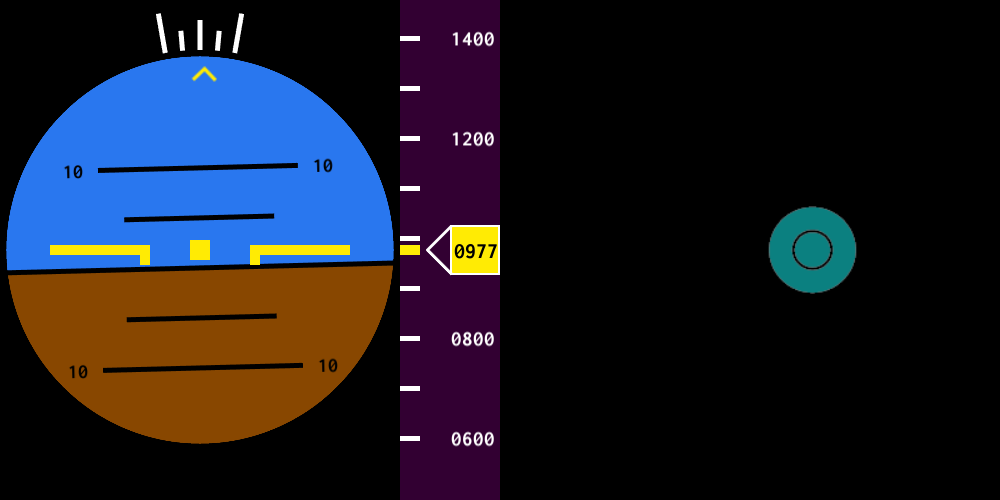
\includegraphics[width=0.8\linewidth]{figures/Aircraft/image1.png}
        \caption[The user interface]{The user interface consisting of the attitude indicator, altimeter, and secondary task.}
        \label{figure-hfes:userinterface}
    \end{center}
\end{figure}

\begin{figure}[b!]
    \begin{center}
        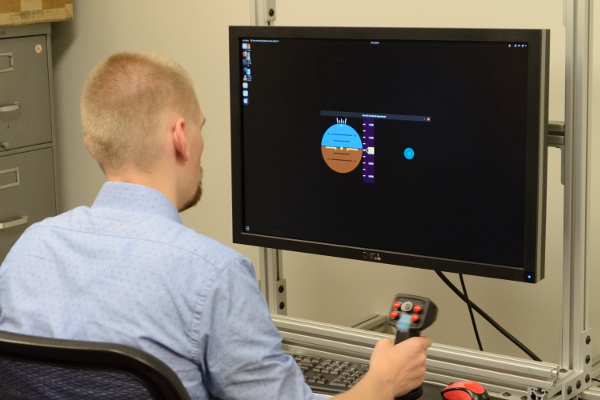
\includegraphics[width=0.8\linewidth]{figures/Aircraft/image2.png}
        \caption[A participant seated in front of the simulator display]{A participant seated in front of the simulator display, controlling the flight task with the joystick.}
        \label{figure-hfes:participant}
    \end{center}
\end{figure}

Participants were seated at a fixed-base simulator for the duration of the experiment, see Figure~\ref{figure-hfes:participant}.
The simulator consisted of a 30-inch monitor and a single joystick.
The user interface was centered in the display and presented to the user at 1000x500 pixels.
The user interface consists of a traditional attitude indicator on the left, an altimeter in the middle, and the secondary task on the right.
The Boeing 747 was modeled using data available in NASA CR-2144~\citep{heffley1972aircraft}.
Flight Condition 2 was chosen for this experiment, and represents slow, sea-level flight, with the landing gear retracted and with flaps extended to 20 degrees.
Longitudinal and lateral body axis derivatives were converted to the stability axis and implemented in a state-space model~\citep{stevens2015aircraft}.
Participants used the elevators and ailerons to control pitch and roll, respectively.
Altitude was controlled by the subject with time-integrated pitch commands, as in a real aircraft.

\subsection{Experimental Design}
Participants were evenly split into two groups: a control group and a feedback group.
Participants in the feedback group received concurrent bandwidth feedback on the first 27 trials (9 in each control mode) and then flew the last 9 trials (3 in each control mode) without feedback to test their immediate retention.
Participants in the control group never received concurrent bandwidth feedback, nor was it mentioned to them during the study.

For participants experiencing feedback, feedback was presented based on the flight control mode of their current trial.
This feedback was implemented by changing the color of an indicator's elements from yellow to red when it deviated from outside of its allowed bandwidth and returning the indicator to yellow when it returned within the bandwidth.
Acceptable bandwidths of 3 degrees for pitch and roll, and 30 feet for altitude were chosen based on preliminary testing.
Pitch feedback occurred on the center dot.
Roll feedback was shown on the wings and the roll indicator at the top of the attitude indicator.
Altitude feedback was enabled on the background color of the altimeter.
In Figure~\ref{figure-hfes:userinterface}, all three parameters are shown inside the acceptable bandwidth, and are therefore displayed in yellow.

Participants began the experiment by signing a consent form, filled out a survey with demographic questions, then had a brief, pre-recorded training session.
After this training, participants immediately began the experiment and progressed through the 36 trials at their own pace.
Participants noted their workload on a piece of paper after each trial.
Subjects in the feedback group were paused after the 27th trial, at which time the proctor explained that the feedback would no longer appear, but that they ``should continue to perform the task to the best of [their] ability.'' Subjects in the feedback group also filled out a questionnaire after the end of the experiment trials which asked them about their experience with the feedback.

\subsubsection{Independent variables}
The three independent variables in this experiment were Group, Mode, and Trial.
Group, a between subjects factor, described if subjects received feedback — Control or Feedback.
Mode, a within subjects factor, was the three different control modes — P, PR, or PRA.
Trial, also a within subjects factor, was the trial that subjects repeated 12 times in each mode.

\subsubsection{Dependent measures}
The root-mean-square error (RMSE) of pitch was calculated for every trial.
This allowed for a consistent measurement across every trial as the same pitch disturbance was present regardless of the control mode.
The roll RMSE was calculated for each PR and PRA trial, and the altitude RMSE was calculated for each PRA trial.
The RMSE values provide an objective measurement of performance.
The secondary task was activated ten times per trial.
Participants had five seconds to correctly respond to the secondary task once it changed color.
We recorded the rates for correct and incorrect responses, as well as lack of response.
We used the average correct response time as objective indication of workload.
The Modified Bedford Workload Scale is a ten-point subjective workload measurement tool~\citep{roscoe_subjective_1990}.
Participants were asked to follow the scale and record their workload after each trial, allowing us to observe changes in workload during training.

\subsection{Hypotheses}
We had three major hypotheses for this experiment:
\begin{itemize}
    \item[\textbf{H1.}] Participants in the feedback group will immediately outperform those in the control group. We expect this effect to be most pronounced for the most complex mode and to see little to no improvement for simple trials.
    \item[\textbf{H2.}] Participants in the feedback group will have lower workload than participants in the control at the end of the experiment. We expect this effect to be most pronounced for the most complex mode and to see little to no improvement for simple trials.
    \item[\textbf{H3.}] Participants in the feedback group will not suffer from the guidance hypothesis and will retain their performance and workload levels when the feedback is removed in the immediate retention trials.
\end{itemize}
These hypotheses were established from the literature, our previous experiments with feedback, and early pilot studies with this simulation framework.

\section{Results}
\subsection{Participants}
Participants in the experiment were 30 engineering students from the University of California, Davis (23 men, M = 23.0 years, SD = 4.4; 7 women, M = 22.6 years, SD = 3.0).
All participants had normal or corrected-to-normal vision and full motor control of their upper bodies.
Eighty percent of participants had previously used a joystick, 43\% had spent time in flight simulators, and 30\% had prior flight experience.
Both gender and participants with flight experience were counterbalanced between the two groups.
Written informed consent was obtained prior to testing in accordance with the University of California, Davis Institutional Review Board.

\subsection{Analysis}
Mixed models were used to calculate the significance of factors in our analysis due to the presence of performance outliers which were removed from the analysis.
The Satterthwaite method was used to calculate the adjusted degrees of freedom using the lmerTest package in R~\citep{RN53}.
When significant effects were observed, post hoc comparisons using the Tukey Honest Significance Difference (HSD) test were performed and considered significant at the p $<$ .05 level, and the Satterthwaite method was again used to calculate the degrees of freedom.
Only 7 of the 1080 total trials (30 subjects with 36 trials per subject) were removed.
These trials were extreme performance outliers, and including these trials does not change the primary results of the study.
A three-factor (Group, Mode, and Trial) mixed model with two repeated measures (Mode and Trial) was run on the pitch root-mean-square error.
There were significant main factors of group ($F(1, 27.97) = 6.3, p = 0.018$), mode ($F(2, 53.47) = 29.7, p < .001$), and trial ($F(11, 300.29) = 48.4, p < .001$).
There were also significant interaction effects between group and trial ($F(11, 300.29) = 2.5, p < 0.01$) and between mode and trial ($F(22, 601.58) = 2.8, p < .001$).
Despite the presence of interaction effects that result from participants learning the task (as indicated by the trial factor), the main effects can still be interpreted, see Figure~\ref{figure-hfes:pitchrmse}.
A Tukey test showed that the participants in the groups differed significantly, with the participants in the feedback group outperforming those in the control group ($M = 2.35, 3.05$, respectively, $SE = 0.20$).
An additional Tukey test showed that the participants' performance in the modes differed significantly, and participants performed best in P mode, followed by the PR mode, and finally the PRA mode ($M = 2.30, 2.67, 3.14$ respectively, $SE = 0.15$).

This same analysis was completed on the roll root-mean-square error, with similar results.
There were significant main factors of group $(F(1, 28.00) = 8.8, p < 0.01)$, mode $(F(1, 27.93) = 6.8, p = 0.015)$, and trial $(F(11, 308.22) = 19.6, p < .001)$.
There was also a significant interaction effect between mode and trial $(F(11, 308.06) = 4.6, p < .001)$, see Figure~\ref{figure-hfes:rollrmse}.
Tukey tests showed that the participants' performance between the groups and the modes each differed significantly, with the participants in the feedback group again outperforming those in the control group ($M = 1.96, 2.43$, respectively, $SE = 0.11$), and performance was best in the PR mode followed by the PRA mode ($M = 2.15, 2.24$, respectively, $SE = 0.08$).
A two-factor (Group and Trial) mixed model with one repeated measure (Trial) was run on the altitude root-mean-square error.
There were significant main factors of group ($F(1, 27.54) = 5.2, p = 0.030$) and trial ($F(11, 301.57) = 11.4, p < .001$).
Tukey tests showed that the participants' performance between the groups differed significantly, with the participants in the feedback group again outperforming those in the control group ($M = 28.3, 50.2$, respectively, $SE = 6.8$), and the trial effect showing learning throughout the experiment for both groups, see Figure~\ref{figure-hfes:altitudermse}.
See Figure~\ref{figure-hfes:completermse} for a plot of the root-mean-square error for each flight task in each mode.
A three-factor (Group, Mode, and Trial) mixed model with two repeated measures (Mode and Trial) was run on the modified Bedford workload scores.
There were significant main factors of mode ($F(2, 56) = 134.8, p < .001$), and trial ($F(11, 308) = 8.7, p < .001$), and a significant interaction effect between mode and trial ($F(22, 616) = 2.0, p < 0.01$).
Tukey tests showed that the participants' workload between the modes differed significantly, with workload lowest in P, then PR, and finally PRA ($M = 3.80, 4.99, 6.16$, respectively, $SE = 0.28$), and the trial effect representing slightly reduced workload throughout the experiment.

\begin{figure}[b!]
    \begin{center}
        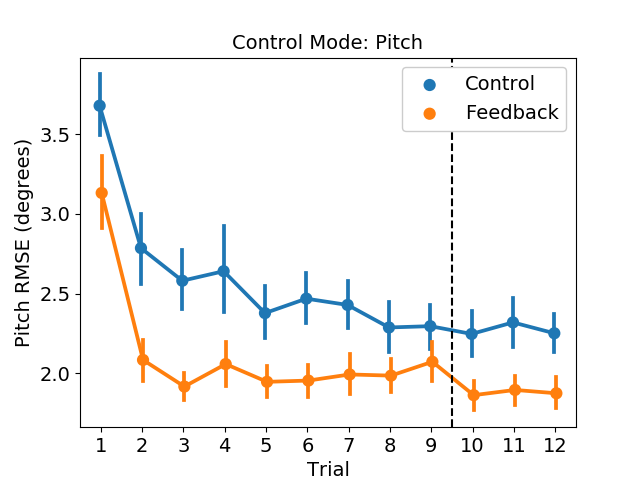
\includegraphics[width=0.8\linewidth]{figures/Aircraft/image3.png}
        \caption[The mean Pitch RMSE for each trial]{The mean Pitch RMSE for each trial for participants in the P control mode. Data points are the mean, and error bars are the standard error of the mean.}
        \label{figure-hfes:pitchrmse}
    \end{center}
\end{figure}
\begin{figure}[b!]
    \begin{center}
        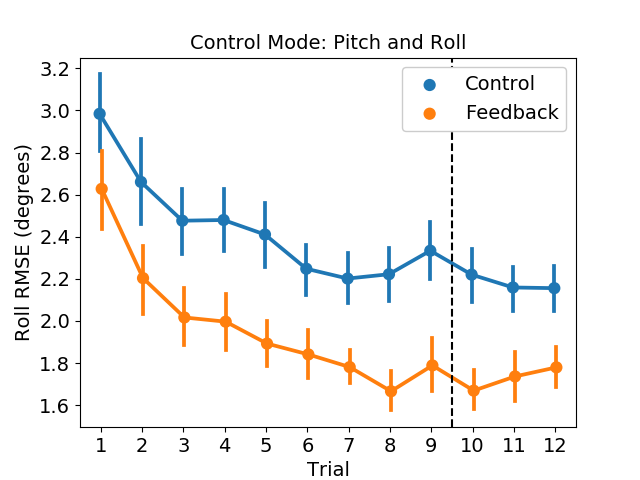
\includegraphics[width=0.8\linewidth]{figures/Aircraft/image4.png}
        \caption[The mean Roll RMSE for each trial]{The mean Roll RMSE for each trial for participants in the PR control mode. Data points are the mean, and error bars are the standard error of the mean.}
        \label{figure-hfes:rollrmse}
    \end{center}
\end{figure}
\begin{figure}[b!]
    \begin{center}
        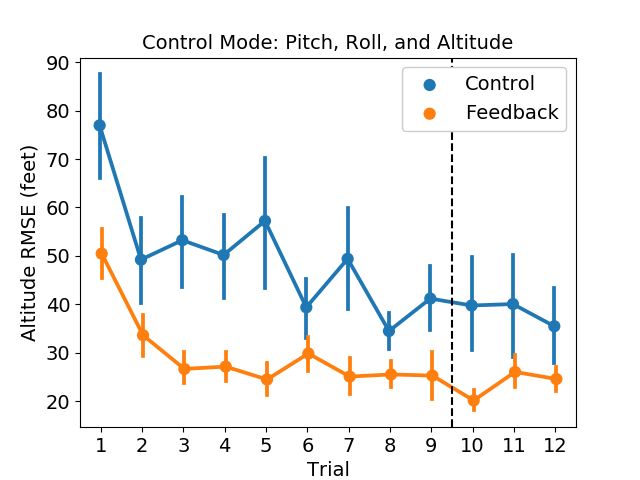
\includegraphics[width=0.8\linewidth]{figures/Aircraft/image5.png}
        \caption[The mean Altitude RMSE for each trial]{The mean Altitude RMSE for each trial for participants in the PRA control mode. Data points are the mean, and error bars are the standard error of the mean.}
        \label{figure-hfes:altitudermse}
    \end{center}
\end{figure}

\begin{figure}[b!]
    \begin{center}
        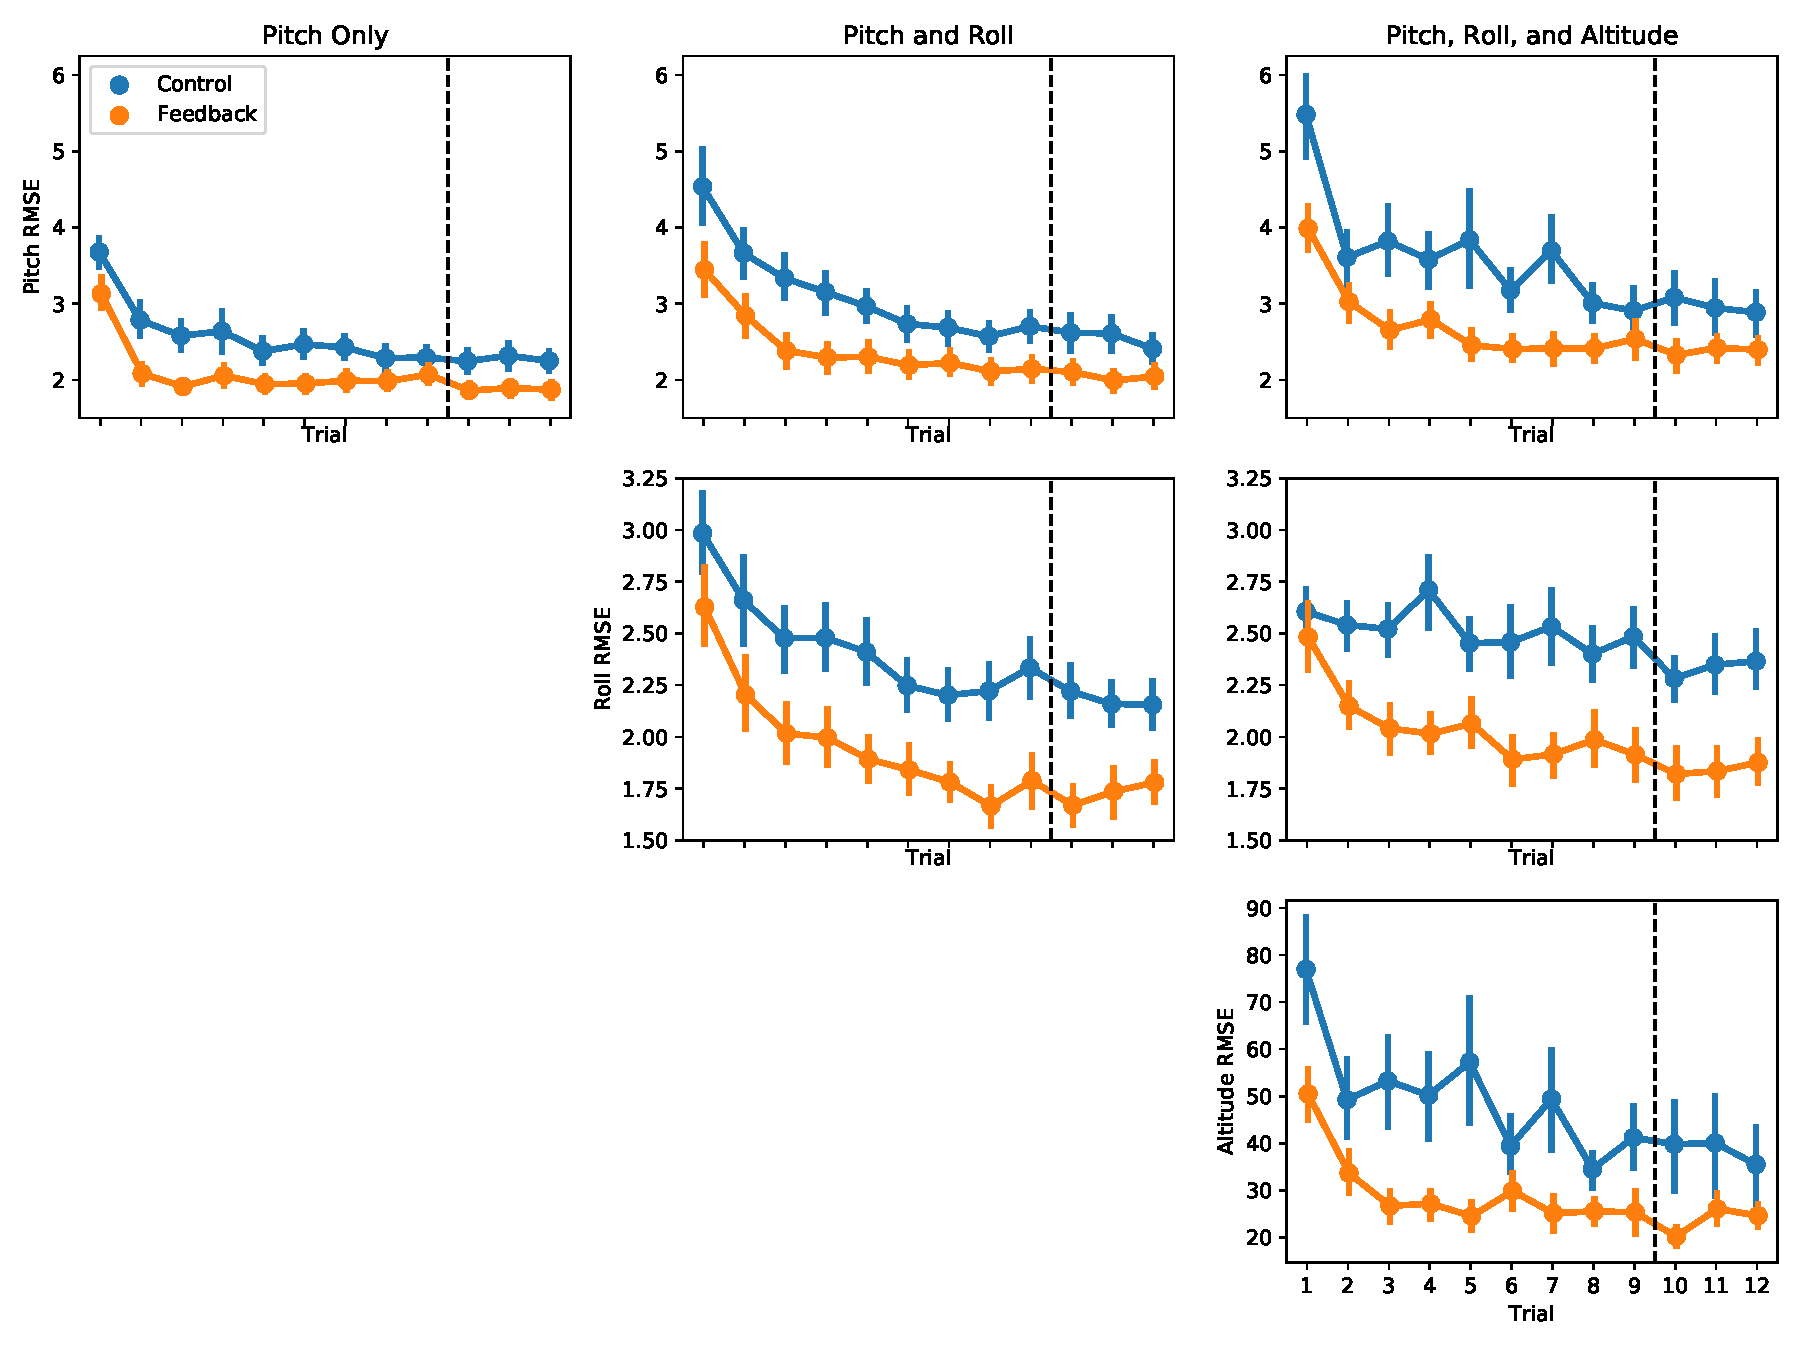
\includegraphics[width=\linewidth]{figures/Aircraft/performance_measures.pdf}
        \caption[The root-mean-square error for each flight task in each mode]{The root-mean-square error for each flight task in each mode. Data points are the mean, and error bars are the standard error of the mean.}
        \label{figure-hfes:completermse}
    \end{center}
\end{figure}

\section{Discussion}

\begin{table}[tb]
    \centering
    \includetable{aircraft-perf-improvement.tex}
    \caption[Performance improvement of the feedback group over the control group]{Performance improvement of the feedback group over the control group at the end of the experiment for each flight RMSE metric.}
    \label{aircraft:perf-improvement}
\end{table}

Our analysis showed that participants in the feedback group performed significantly better than the control group in every trial across every metric and flight control mode.
For the first time that participants completed P, PR, and PRA trials, the feedback group performed 17.5\%, 31.7\%, and 37.4\% better than the control group according to the pitch RMSE metric.
Participants in the feedback not only immediately performed better, they also reached their peak performance much faster and had a final performance level which was significantly better than the control group, see Table~\ref{aircraft:perf-improvement}.
The largest performance improvement was seen in controlling altitude, where the feedback group had a final performance level which was 44.2\% better than the control group, confirming H1.
No group-related workload differences were detected in either the Modified Bedford scores or in the secondary task reaction times.
This suggests that, for tasks of this complexity, concurrent bandwidth feedback may not reduce workload~\citep{karasinski_evaluating_2019}.
Thus, for our second hypothesis, H2—we find that concurrent bandwidth feedback does not reduce workload in our flight tasks, and that tasks with higher functional complexity may be required to observe these effects.
Our third hypothesis was that subjects would primarily use the concurrent bandwidth feedback as a learning tool but that they would not become dependent on the feedback to the point that they required it to complete the task.
Retention tests are commonly used in the augmented feedback literature to verify that participants are not dependent on the feedback techniques.
Our analysis indicates no significant performance changes across any of our performance metrics when the feedback was removed, confirming H3.
After the experimental trials, we asked participants in the feedback group to complete a survey designed to identify when the feedback was or was not useful and how participants thought their performance and workload changed in the retention phase of the experiment.
One hundred percent of participants thought that the feedback helped them perform the task, 80\% reported that it helped them regain focus when their mind wandered, 73\% reported that it helped them to learn a scan pattern, and 27\% reported that the feedback was motivating.Survey results suggested that participants found the feedback especially useful in the roll and altitude tasks, which was reflected in the objective performance metrics.

\section{Conclusions}
Participants took part in a study investigating the effect of concurrent bandwidth feedback on flight performance and workload in three flight control modes of increasing complexity.
The participants in the feedback group performed significantly better than those in the control group, generally performing better on their second trial than those in the control group could by the end of the experiment.
Subjective and objective workload metrics showed no change in participant workload between the groups.
Survey questions identified that most participants found the feedback helpful in training them to establish a scan pattern, helping them to learn the task much quicker than those without feedback.
Feedback was removed for immediate retention trials, and participants showed no changes in performance or workload, suggesting that participants did not suffer from the guidance hypothesis.
